% -------------------------------------------------------------------------------------
% Plantilla de un art�culo para publicar en la Revista Colombiana de Estad�stica
% *************************************************************************************
% -------------------------------------------------------------------------------------
% Establecer primero el idioma principal del art�culo, por defecto es espa�ol; para
% utilizar otro idioma, cambiar el comando "\documentclass{revcoles}" por el comando
% "\documentclass[english]{revcoles}" o por "\documentclass[portuguese]{revcoles}"
% **** --------------------------------------------------------------------------------
\documentclass[project,twoside,english]{revcoles}
\labeldocument[
university = University of Warwick,
faculty = Centre of Complexity Science,
year = 2015,
]
%department = Departamento de Estad�stica,
%program = Carrera de Estad�stica,
%subject = Estad�stica descriptiva multivariada,
%city = Bogot�,
%month = 4,

% -------------------------------------------------------------------------------------
% Espacio reservado para la carga de los paquetes por parte del autor
% **** --------------------------------------------------------------------------------

\usepackage{listings}





% //// --------------------------------------------------------------------------------
% -------------------------------------------------------------------------------------
% Espacio reservado para colocar las definiciones especiales por parte del autor
% **** --------------------------------------------------------------------------------




% //// --------------------------------------------------------------------------------
% -------------------------------------------------------------------------------------
% Espacio utilizado para colocar las palabras que necesitan partici�n sil�bica
% **** --------------------------------------------------------------------------------
%\hyphenation{Colombia mul-ti-va-ria-do pro-ba-bi-li-dad es-ta-d�s-ti-ca}
% //// --------------------------------------------------------------------------------
\begin{document}
% -------------------------------------------------------------------------------------
% Espacio reservado para ingresar el t�tulo del art�culo
% "maintitle = " t�tulo original del art�culo
% "secondtitle = " t�tulo del art�culo traducido al idioma alterno
% "shorttitle = " t�tulo corto (opcional) para el encabezado
% **** --------------------------------------------------------------------------------
\title[maintitle = The evolution of Zipf's coefficient and the kernel lexicon in six European languages.]
       %secondtitle = Template for report in a course,
       %shorttitle = Plantilla para edici�n de trabajos de cursos

% //// --------------------------------------------------------------------------------
% -------------------------------------------------------------------------------------
% Espacio reservado para ingresar el(los) autor(es) del art�culo de forma individual.
% opci�n "firstname = " nombres completos de cada autor
% opci�n "surname = " primer apellido de cada autor
% opci�n "numberinstitution = " n�mero que identifica la instituci�n a la que pertenece
%         el autor, en caso de haber solo una instituci�n el campo se elimina
% opci�n "affiliation = " afiliaci�n o cargo que desempe�a el autor en la instituci�n
% opci�n "email = " direcci�n electr�nica del autor (preferiblemente institucional)
% **** --------------------------------------------------------------------------------
\begin{authors}
\author[firstname =David,
        surname = Pardo]
        %code = C�digo: 160000,
        %email = cepardot@unal.edu.co,

\author[firstname =Thomas ,
        surname =  Hills]
      %  code = C�digo: 160001,
       % email = eccubidesg@unal.edu.co

\end{authors}
% //// --------------------------------------------------------------------------------
% -------------------------------------------------------------------------------------
% Espacio reservado para ingresar la informaci�n de la(s) instituci�n(es) a la(s)
% cual(es) pertenece(n) el(los) autor(es)
% Usar un comando "\institute"  por cada una de las diferentes instituciones.
% Los campos "subdivision" y "division" son opcionales
% Los campos "institution", "city" y "country" son obligatorios
% **** --------------------------------------------------------------------------------
%\begin{comment}
%\begin{institutions}
 %    \institute[subdivision = Departamento de Estad�stica,
%                division = Facultad de Ciencias,
%                institution = Universidad Nacional de Colombia,
%                city = Bogot�,
%                country = Colombia]
%\end{institutions}
%\end{comment}
% //// --------------------------------------------------------------------------------
% -------------------------------------------------------------------------------------
% CUERPO DEL DOCUMENTO
% **** --------------------------------------------------------------------------------
% -------------------------------------------------------------------------------------
% Espacio reservado para colocar el resumen en el idioma principal y las palabras clave
% !!No dejar salto de l�nea entre el resumen y el comando \keywords{.}��
% **** --------------------------------------------------------------------------------
%%\begin{comment}
\begin{mainabstract}
The evolution of six European languages over the last two centuries is studied by calculating Zipfian power-law coefficients of word occurrences per year in the Google 1-grams. Two coefficients are analyzed, corresponding to the kernel and unlimited lexicons. The former, related to Zipf's coefficient, is shown to have an increasing trend, whereas the latter does not exhibit any discernible pattern. The kernel lexicon is found to have a fairly constant size in terms of number of distinct words, but its proportion with respect to the whole lexicon regarding the number of tokens is found to be linearly decreasing. It is hypothesized that an increase in the topicality of language can explain the observed phenomena.
\end{mainabstract}
%%\end{comment}
% //// --------------------------------------------------------------------------------
% -------------------------------------------------------------------------------------
% Espacio reservado para colocar el resumen en el idioma secundario y las palabras clave
% !!No dejar salto de l�nea entre el resumen y el comando \keywords{.}��
% **** --------------------------------------------------------------------------------
%\begin{comment}
%\begin{secondaryabstract}
%This document gives the instructions to prepare a \LaTeX\ version of the graduation project of undergraduate in
%Statistics to first semester of 2008. The document is written using a \LaTeX\ format (file \emph{Plantilla para trabajo
%de grado.tex}) and can be used as a guideline just replacing its contents. It is necessary to use also the files
%\emph{revcoles.cls}, \emph{references.bib} and \emph{graph\_example.eps}.
%
%\keywords{\LaTeX\ format for documents, undergraduate in Statistics}
%\end{secondaryabstract}

%\end{comment}% //// --------------------------------------------------------------------------------
% -------------------------------------------------------------------------------------
% T�tulo de la primera secci�n
% **** --------------------------------------------------------------------------------




\section{Introduction}
 
  
 Language is one of the features that have let humans develop the varied and complex societies witnessed by history. It has set us apart from other species by making possible the transmission of all kind of ideas in an effective and clear manner. Being at the heart of our ever changing cultures, it evolves constantly, subject to all the influences experienced by humans, in such a degree that we can notice differences in language characteristics between neighboring towns and even within cities. With over 6000 different languages distributed across 200 families it could be surprising to find general commonalities, although they all arise from the same organic structure, namely our brain, and thus share inherent constraints and properties.\\
 
The study of language as a complex system can allow us to find common features and delve into the possible explanations of language behavior. From complex networks theory to data analysis, language can be probed using different tools to obtain information on different levels, such as the storage of words in memory, the network of words and meanings in the brain, or the statistical features of texts and dialogues. Interrelations among all the different phenomena are also of interests, since specific features of one level could be explained as a consequence of a trivial fact of another, e.g. the number of words an author can memorize will have a direct effect on the texts she will produce.\\

The main objective of the present work is to study the evolution of languages. A fundamental requirement for linguistic studies which is not always available is data; taking into account that language is produced everyday in overwhelming amounts, this is difficult to believe. However, if we think about the times before computers, i.e. almost the entire human history, all the relevant data was collected in books, which is not the most convenient format to perform data analysis. Hence, Google n-gram dataset, consistent of word occurrence counts per year in what was claimed to be approximately 4\% of books ever published \cite{Culturomics}, is an invaluable resource for any attempt on investigating the behavior of language in the last few centuries. This will be our main asset in the current study and thus, it will focus on the evolution over the last 200 years of six of the eight languages provided in the dataset, namely English, German, Russian, Spanish, French and Italian. Chinese and Hebrew were discarded because of time and computer limitations, so that we restrict our study to a group of related languages whose evolution should be directly comparable. \\

This enormous dataset has been used to study different aspects of culture and language evolution, in a field now called "Culturomics". \citeasnoun{Culturomics} not only made the data available, they also studied cultural trends, the evolution of grammar, epidemiology, among others, based on the changes in occurrences of certain words over the years. \citeasnoun{death} analyzed the rates of birth and death of words, which were shown to follow decreasing and increasing trends respectively, as well as long term word correlations, which were used to give a measure of cultural memory. Aspects of the evolution of psychology as world population moved from rural to urban lifestyles were scrutinized in a paper by \citeasnoun{psychology}. As a final example of the broad range of topics investigated using Google n-grams, we introduce the main reference for the present study, i.e. \cite{cool}, where the authors analyse statistical characteristics of language over the last two centuries, and conclude that there is a slowdown in linguistic evolution in terms of the annual growth fluctuations of word use.\\
   
In the present work we will focus on one of the most studied properties in quantitative linguistics, i.e. Zipf's law for words \cite{Zipf}. Not really a law, but an empirical observation, it states that the frequency of a word $f$  is inversely proportional to its rank $z$, following a relation of the form
\begin{equation}
f(z)\sim z^{-\zeta},
\end{equation}

with $\zeta \approx 1$. This is not an exclusive feature of language, since similar empirical results have been found regarding the size of cities \cite{cities}, distribution of words in programming languages \cite{programming}, the distribution of incomes in a nation \cite{income}, among many others. Furthermore, it is just a rough approximation, with better fits having been obtained for more complex models, such as the Zipf-Mandelbrot law \cite{mandelbrot}, log-normal models or a generalized Z-distribution \cite{Baayen}. However, \citeasnoun{Baayen} also showed that the best fitting distribution depends on the specific text analysed, and there is no single model that can account for all subtleties of language. More information on Zipf's law variation across languages can be found in \cite{zipf-variation} and a very complete review on the topic is given in \cite{review}, which includes analysis of different plausible models of its emergence. \\

\section{Methodology}

Taking into account that we are interested in studying the evolution of language behavior over two centuries, it is useful to consider a model with the least number of parameters possible that can nevertheless explain an important part of the observations. In this way we can focus on fitting only a few parameters and observe how their value changes over time. With this consideration in mind, it was decided to follow the approach of \citeasnoun{cool}, based on a model proposed in a paper by \citeasnoun{regimes}. The authors of the latter found that for sufficiently large texts ($588030$ different words in their case) the data can be fitted by two different power-laws for different frequency regimes, i.e. the original Zipf's law for the most frequent words, called "kernel lexicon", and a steeper slope for the rarer words, named "unlimited lexicon". The kink which demarcates the transition between the two regimes was found to be in the range of words ranked between $5000$ and $6000$. \\

\citeasnoun{cool} didn't calculate Zipf's coefficient itself, but the related coefficients of the probability density function 

\begin{equation}
P(f)\sim \left\{
     \begin{array}{ll}
       f^{-\alpha_{-}}, & \text{if } f<f_{\times} \text{ (unlimited lexicon)}\\
       f^{-\alpha_{+}}, &\text{if } f>f_{\times} \text{ (kernel lexicon)}.\\
        
     \end{array}
   \right.
\end{equation}



This avoids possible correlations between rank and frequency that can affect the statistical fitting of a power law to the data; moreover Zipf's coefficient can still be estimated due to the asymptotical relation \cite{regimes}

\begin{equation}
\alpha_{+}\approx 1+\frac{1}{\zeta}.
\end{equation}

In their study, \citeasnoun{cool} established the limits for the regimes a priori, and they calculated the best fit for a power-law for the selected regions. In this way they obtained  $\alpha_{+}\approx 2$ and $\alpha_{-}\approx 1.7$ over all languages (Figure \ref{Regimes}  illustrates the two regimes for English in the year 2000). They also found averages and standard deviations for this values over the period 1800-2008 for each language separately. Nonetheless, they did not consider the evolution of this coefficients nor the possibility of a variability in the kink.\\


\begin{figure}[!htb]
  \centering
  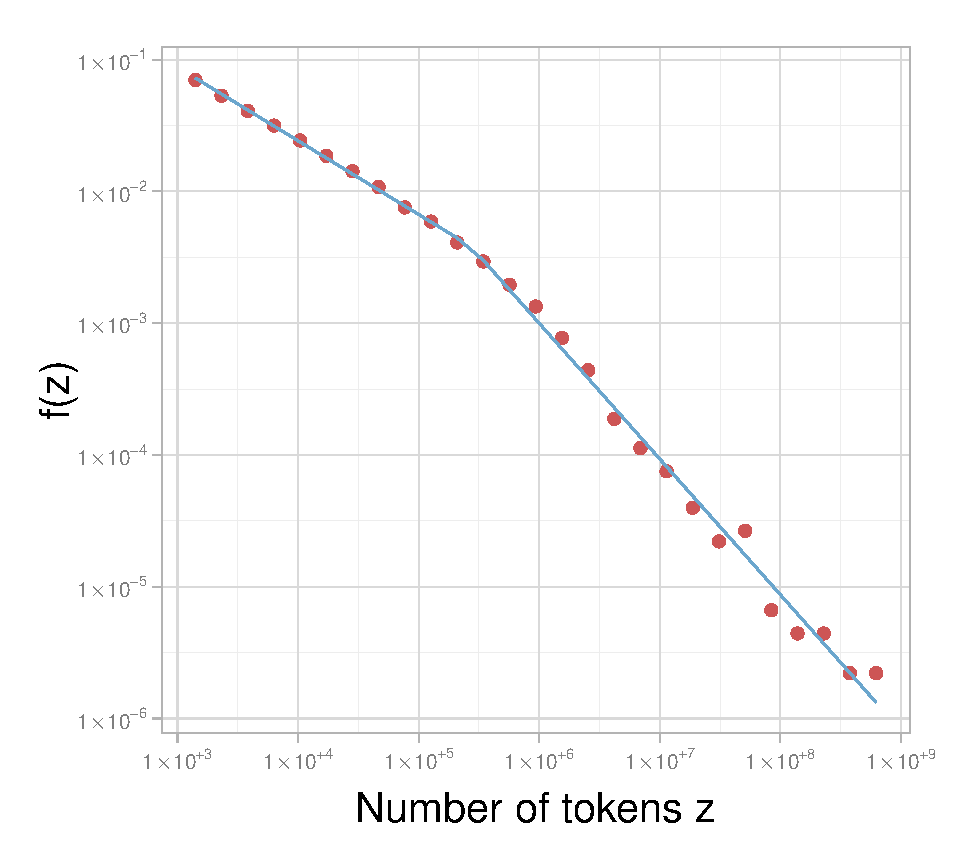
\includegraphics[scale=0.6]{Regimes.eps}
 \caption{Frequency vs Number of tokens for English in the Google 1-grams for the year 2000. Two different power law regimes can be observed, with a kink present in the transition between them. Zipf's original law only holds for the most frequent words, that is, where the distribution is steeper. }
   \label{Regimes}
\end{figure}


In order to investigate one component of language evolution we decide to fill this gap, dilucidating whether Zipf's coefficient, or more specifically the related $\alpha_+$, has followed any evolutionary trend. Besides, we also delve into the possibility of a variability in the kernel lexicon, instead of fixing its limits according to previous results. A maximum likelihood method proposed by \citeasnoun{Clauset} is used to obtain the coefficient of the best power-law fit for the data; this algorithm has the particularly attractive feature that it identifies a lower bound for the power law, that is, the frequency for which the fitting starts being statistically significant. Thus, we automatically obtain a limit for the kernel lexicon, and the data outside the corresponding region, the unlimited lexicon, is fitted again to obtain the information of the second regime.\\

The data to which the algorithm is applied is a filtered version of the original Google 1-grams; the original data has one row per word per year indicating its number of occurrences, which we transform in a table in which each row contains a word, one column per year giving its number of occurrences and one last column for the total number of occurrences. Words containing numeric values and symbols different from letters and accents are removed, as well as those words for which the counts are less than $50$ for all years; this is done with the intention of removing typos and entities with no meaning. Furthermore, each time a word has less than 50 counts, it is removed from the dataset for that year. This ensures that extremely rare words and typos are filtered out of the data. Although some information might be lost, it is almost certain that the fitting of the power laws won't consider the rarest words, thus our procedure does not affect the results yet makes the dataset more manageable.\\



 
 \section{Results}
 
 One of the most evident  ways in which languages evolve is by growing; in terms of the semantics it is important to consider the number of distinct words, i.e. types, since they are a direct measure of the size of a language. When documents are considered, it is also relevant to study the total number of words in them, not necessarily distinct, which are referred as tokens (For example in the expression \textit{home sweet home} there are two types, \textit{home} and \textit{sweet}, but three tokens). In Figures \ref{types} and \ref{tokens} we observe the exponential increase in the number of types and tokens in the Google 1-grams over the last two centuries. This does not necessarily imply that language has grown exponentially, since the number of documents produced and available for scanning is a determinant factor. Thus, we want to study variations in language that cannot be completely explained by this growth of texts and number of words.\\
 
 \begin{figure}
\centering
\begin{minipage}[t]{.48\textwidth}
  \centering
 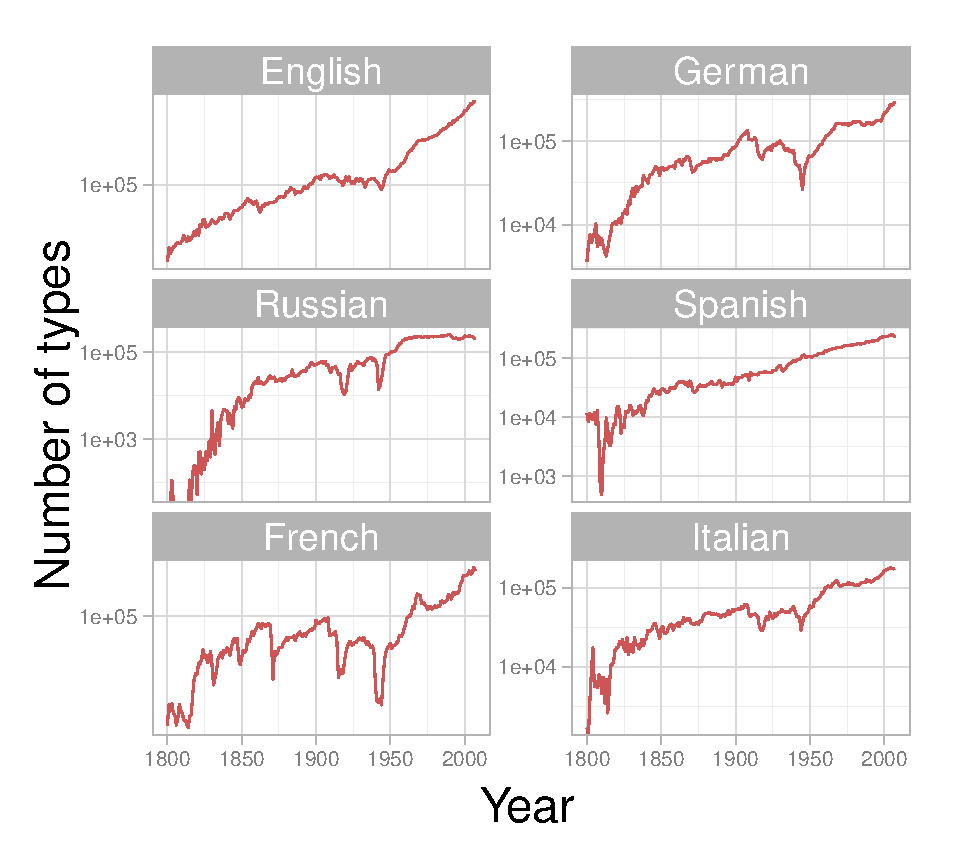
\includegraphics[width=0.9\linewidth]{types.eps}
  \captionof{figure}{Evolution of the number of types in logarithmic scale. An exponential growth is observed, with the curves presenting noticeable dips for important historical, mainly of political and social turbulence, events such as both World Wars or different french revolutions. }
  \label{types}
\end{minipage}%
\hfill%
\begin{minipage}[t]{.48\textwidth}
  \centering
   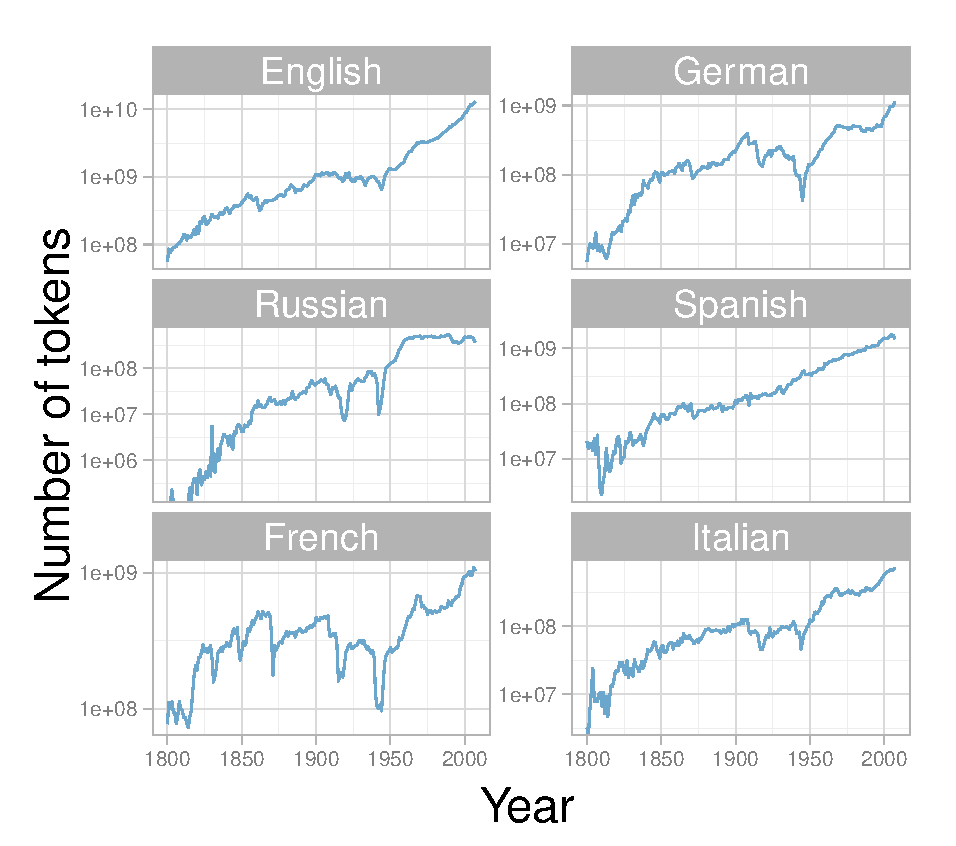
\includegraphics[width=0.9\linewidth]{tokens.eps}
  \captionof{figure}{Evolution of the number of tokens in logarithmic scale. The behaviour resembles the one for types, but with a faster growth.}
  \label{tokens}
\end{minipage}
\end{figure}

\subsection{The kernel lexicon}
 
 Figure \ref{CoefKer} shows the evolution of the coefficient $\alpha_{+}$ for all the analyzed languages; it is observed that there is a general ascending trend, with the coefficient  
 increasing by about $0.1$ for each language over the timespan considered. French is the only language for which this behaviour is reversed in the last years, with the coefficient descending and getting closer to its original value. In the case of German a dip appears in the year 1925, but the coefficient recovers its growing tendency. Some pathological data were removed, mainly in German and Russian, in order to have a plot scale in which the changes are noticeable. In Russian and mainly in English we observe that the coefficient remains constant up to a tipping point, around the beginning of the 20th century, after which it starts increasing. This behavior is equivalent to a decrease in Zipf's original coefficient, which represents a flattening of the relation between rank and frequency of words. This means that the frequencies of adjacently ranked words are getting slightly closer to each other in the kernel lexicon. One can interpret this result as language becoming less predictable, because a leveling of the frequencies directly implies more similar chances of selecting the next word for a text (probabilities being taken according to the frequencies of words).\\
 
 We also obtain information about the lower bound of the data that fits the distribution, which we call the kink, since it corresponds to the point of change between the two power-law regimes. As seen in Figure \ref{kink} the frequency at which this happens tends to be on the order of $10^{-5}$, which gives a bigger kernel lexicon than the one considered by \cite{cool}, were the limit was set at the frequency $10^{-4}$. Furthermore, it can be noticed that, apart from the Spanish case, the kink behaviour is not constant and its evolution exhibits structures similar to the evolution of the coefficient $\alpha_{+}$, more evidently in English and German. In the latter case we observe that the years for which the kink is detected at a much lower frequency correspond to the removed pathological values for the coefficient. However, even though the structures are similar, the general trend is not ascendant, thus the results obtained cannot be explained only in terms of the change in lower bound.\\
 
 \begin{figure}
\centering
\begin{minipage}[t]{.48\textwidth}
  \centering
 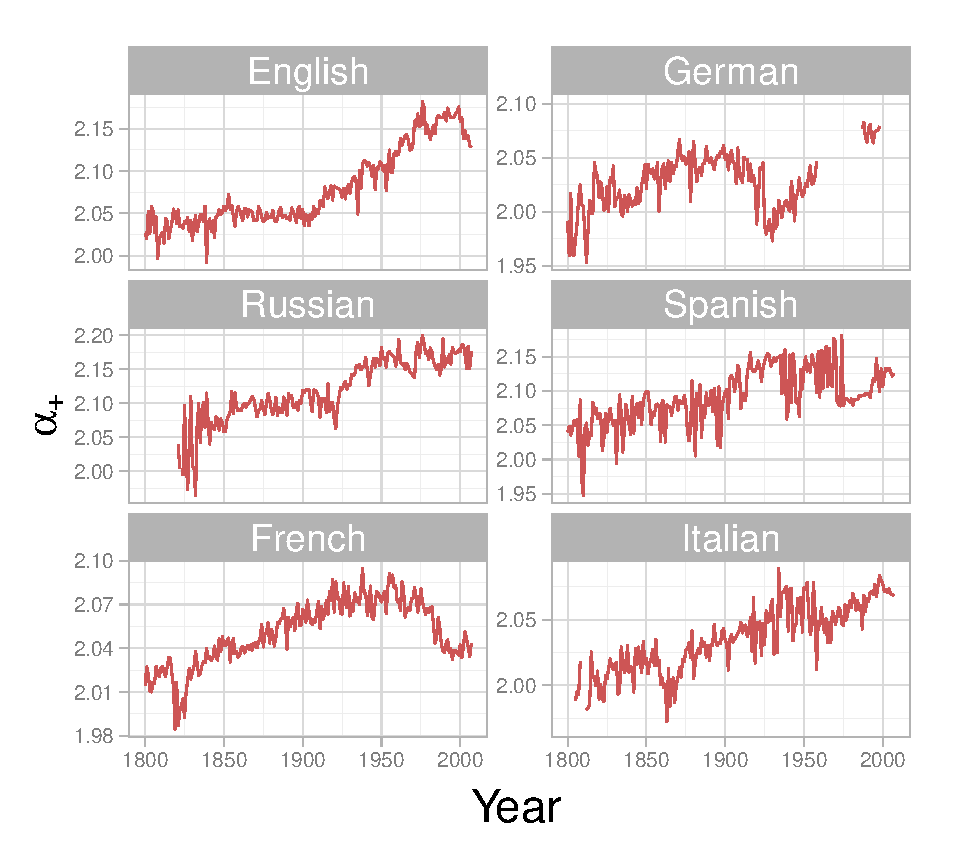
\includegraphics[width=0.9\linewidth]{CoefKer.eps}
 \caption{Evolution of $\alpha_{+}$. A general ascending trend is observed for all languages except french.}
   \label{CoefKer}
\end{minipage}%
\hfill%
\begin{minipage}[t]{.48\textwidth}
  \centering
  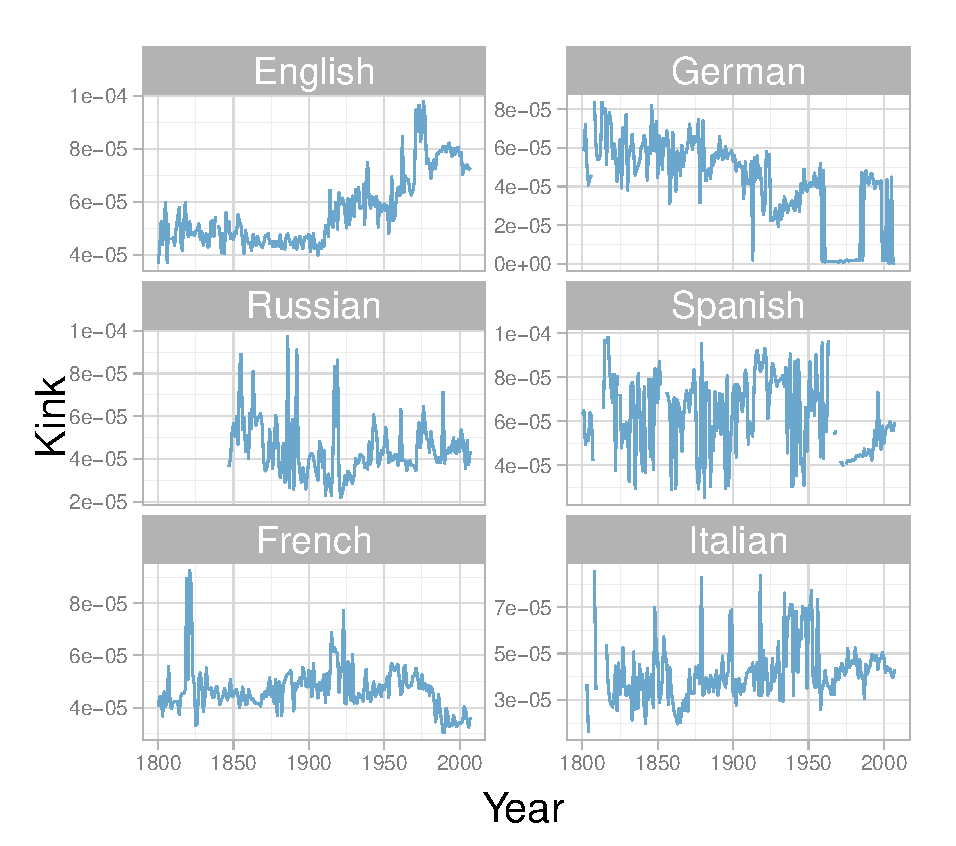
\includegraphics[width=0.9\linewidth]{Kink.eps}
  \captionof{figure}{Evolution of the lower bound frequency for the power-law fitting (the kink). No common pattern is observed across languages, although the local behavior of the time series resembles the ones obtained for $\alpha_{+}$.}
  \label{kink}
\end{minipage}
\end{figure}

Delving more into the features of the kernel lexicon, Figure \ref{abstypes} shows the evolution of its size in terms of the number of types. Although it is a highly noisy signal, it can be seen that in general the number of distinct words in the kernel lexicon remains constant, being around 2500 types, as can be seen in more detail in Table \ref{tabla}. This result agrees with the hypothesis proposed by \citeasnoun{regimes} stating that the kernel lexicon corresponds to the fundamental vocabulary we use to construct meaning and that its size is related with brain constraints, which would explain the similarity in sizes between languages. Nevertheless, when we analyse the size in terms of the number of tokens, an interesting result arises: the proportion of tokens in the kernel lexicon has declined in an approximately linear fashion as we can see in Figure \ref{reltokens}. In more detail, even though the number of types remains constant and there is no general trend in the location of the lower bound for kernel lexicon, its size with respect to the unlimited lexicon has decreased considerably. This brings up the question whether eventually the distinction between this two lexicons could become blurred. If the kernel lexicon effectively owes its existence to certain brain features, we would expect this lexicon to keep being important and representing a considerable fraction of our language production. In spite of this, it is very interesting to see the increasing relevance of the unlimited lexicon over the last couple of centuries.\\ 

 
 \begin{figure}
\centering
\begin{minipage}[t]{.48\textwidth}
  \centering
  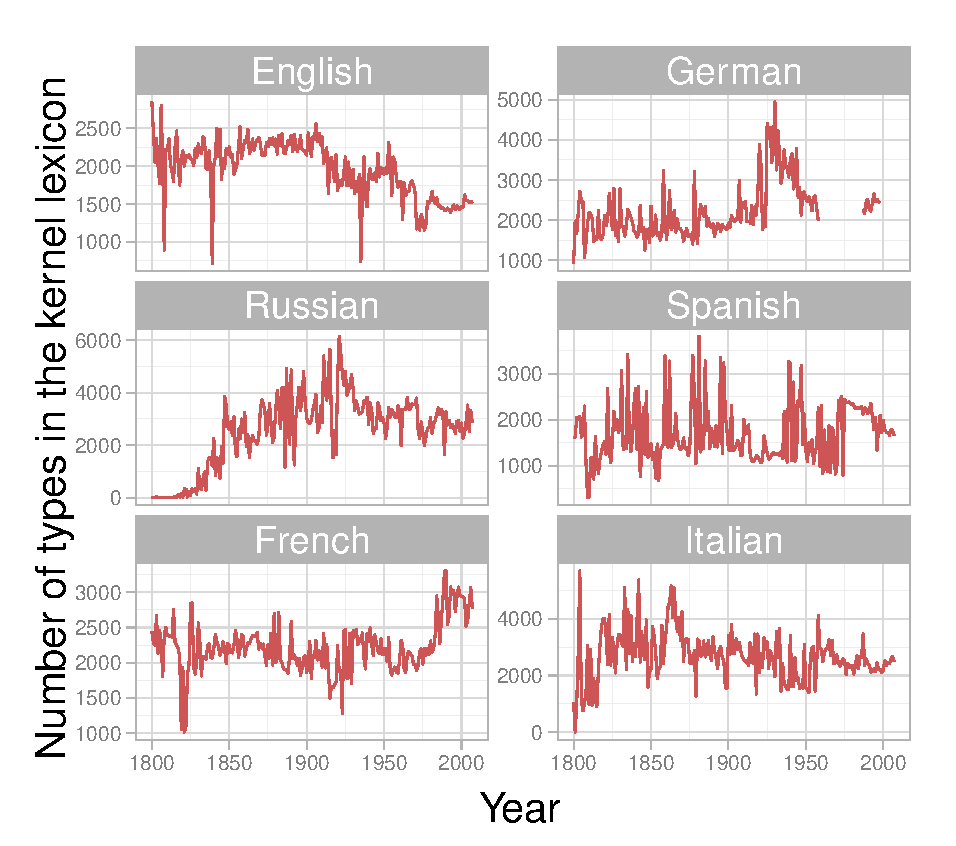
\includegraphics[width=0.9\linewidth]{SizeKer.eps}
  \captionof{figure}{Evolution of the number of types in the kernel lexicon. Although with high variation in a year by year basis, the general sizes of kernel lexicons tend to be centered around a constant value.}
  \label{abstypes}
\end{minipage}%
\hfill%
\begin{minipage}[t]{.48\textwidth}
  \centering
  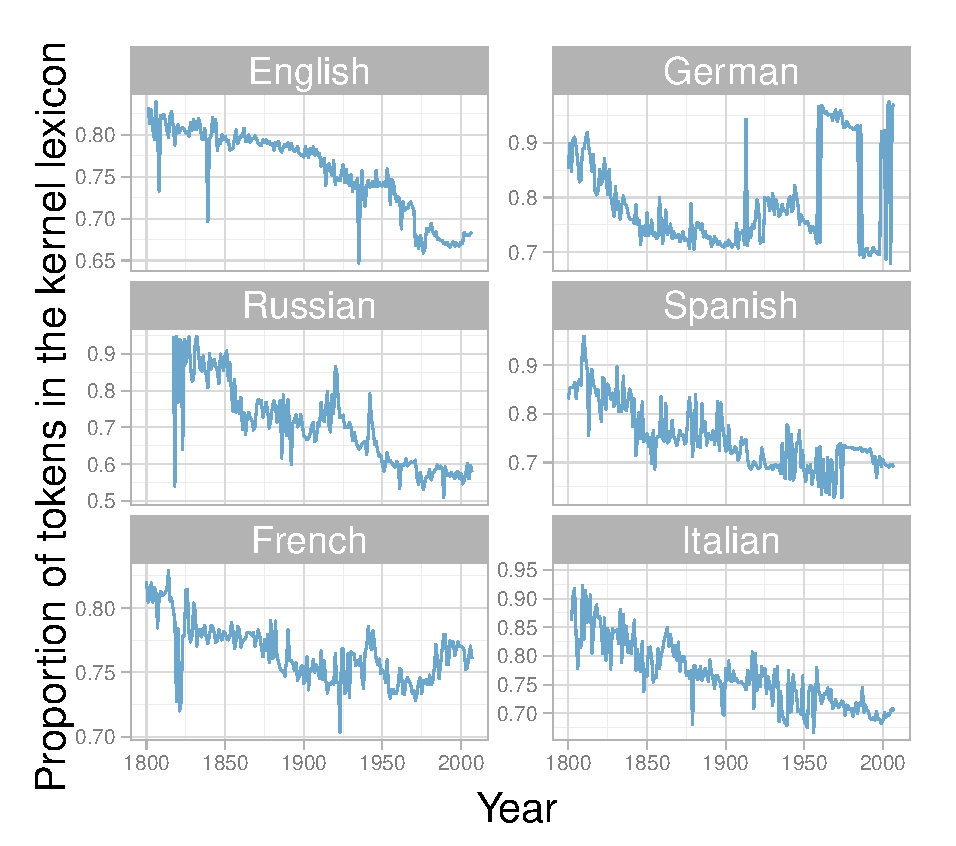
\includegraphics[width=0.9\linewidth]{RelKer.eps}
  \captionof{figure}{Evolution of the proportion of tokens in the kernel lexicon. A decreasing linear trend is observed for all languages.}
  \label{reltokens}
\end{minipage}
\end{figure}

\subsection{Size effects}

We want to study the importance of the growth of the collected data in explaining the trends seen in the power law coefficient and in the kernel lexicon, since the size of texts have been shown to influence Zipf's law \cite{size}. Our first approach consists in analyzing the obtained data as time series, calculating the cross-correlation coefficient between $\alpha_{+}$ and three important and plausibly explanatory variables. These are the total number of types, the total number of tokens and the lower bound for the power law expressed in terms of number of tokens. The cross-correlation coefficient without time lags is simply the correlation between the variables, i.e.

\begin{equation}
r_{xy}=\frac{\sigma_{xy}}{\sigma_x\sigma_y}.
\end{equation} 

The results, summarized in Table \ref{tabla}, show a high correlation between $\alpha_{+}$ and all the variables for English, German, Russian and Italian. For Spanish the correlations are around $0.5$ and for French they are low, which indicates that there are other factors in play besides the increasing numbers of types and tokens. Since all languages come from the same family and are mainly spoken in countries that share historical and cultural circumstances, it can be argued that the mechanisms that have a big effect in French and Spanish should also be at work for the other four cases, although with less impact.\\

\begin{figure}
\centering
\begin{tabular}{| l | c | c | c | c |}
  \hline
  Language & Size &Types & Tokens & Kink \\
  
  \hline                       
  
  English & 1958 & 0.850 & 0.745 &  0.767 \\
  German & 2230 & 0.612 &  0.605  & 0.753  \\
  Russian & 2528 & 0.762 & 0.706 & 0.711\\
  Spanish &1695 & 0.490 & 0.377 & 0.537\\
  French & 2218 & 0.225 & 0.112 & 0.260\\
  Italian & 2685 & 0.708 & 0.648 & 0.724\\
  \hline  
\end{tabular}
\captionof{table}{Average number of types in the kernel lexicon and cross-correlation coefficients of the total number of types, total number of tokens and the lower bound of the power law with respect to $\alpha_{+}$ for all languages.}
\label{tabla}
 \end{figure}
 
 In order to corroborate that size effects are not entirely responsible for the behavior of the coefficients, we use $100$ bootstrap samples of one million words extracted with replacement and with probabilities proportional to the original frequencies of the words. Moreover, we use the maximum likelihood method for fitting the power law only for the $2000$ most popular words, that is approximately the size of the kernel lexicon, to discard effects that the tail of the distribution might produce. In this way we eliminate two size influences, by fixing the total number of types and tokens.\\
 
 In Figure \ref{Boots} we show one box plot per year, such that each vertical red line gives the range of the obtained bootstrapped data, except for the outliers which are shown as black dots. The trends observed previously are preserved, confirming that size effects have limited influence and cannot explain all the variation in the coefficients. Moreover, the ill-behaved data, such as the 1960-1980 range in German disappear, probably because the range for the lower bound was fixed. \\
 
 \begin{figure}[!htb]
  \centering
  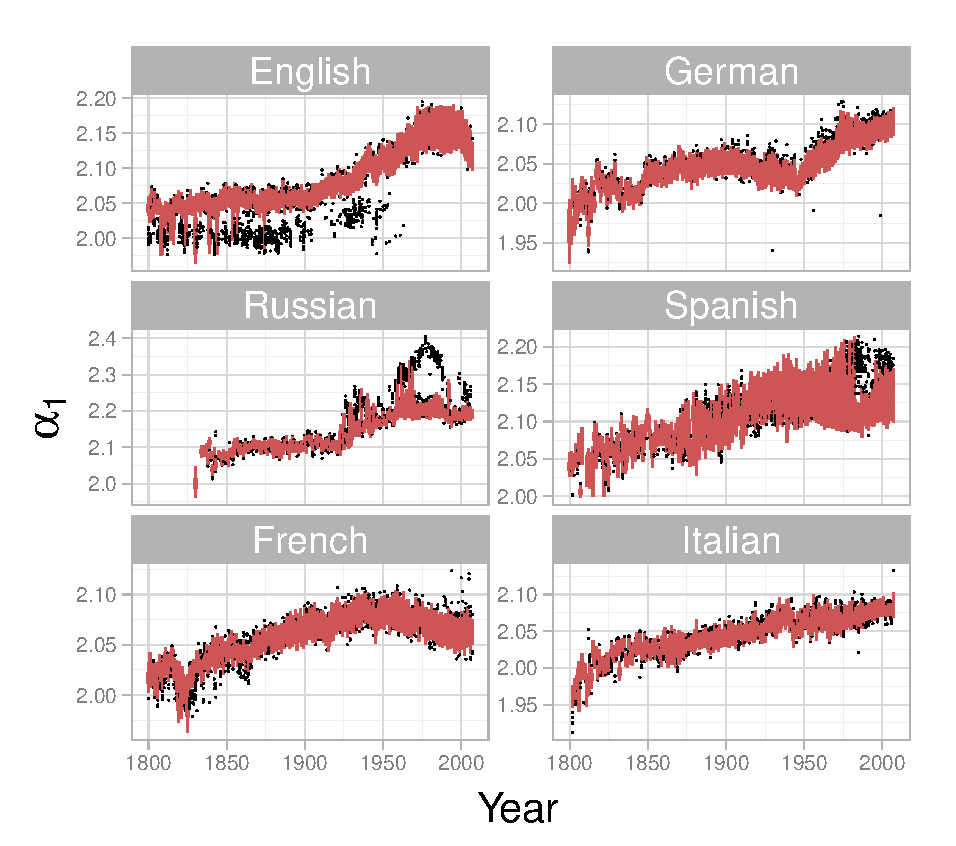
\includegraphics[scale=0.6]{Bootstrap.eps}
 \caption{Evolution of $\alpha_{+}$ calculated using 100 bootstrap samples per year. The trends observed using the complete dataset are preserved. }
   \label{Boots}
\end{figure}

\subsection{The unlimited lexicon}

Different methods were used to tackle the analysis of the unlimited lexicon. First of all \citeasnoun{Clauset}'s algorithm was used over a new dataset corresponding to all the words outside the kernel lexicon. This approach yielded statistically significant results for only the most recent years and the obtained coefficients varied mainly between 1 and 3, which is to broad a range to be of any interest, see Figure \ref{alphamin}. The cause of this is probably that the obtained fitted power law is based on data on the transition region between the two lexicons. Hence, they do not reflect the real behaviour of the unlimited lexicon, but that of a region in which the data has become large enough in recent years to be detectable by the algorithm.\\

Then, following \citeasnoun{cool} we selected a fixed range for the unlimited lexicons, namely those words with relative frequencies below $10^{-5}$. The number of statistically significant fits was even lower than in the previous case, and similarly with a broad range for the coefficients, as is illustrated in Figure \ref{alpha-5}. The explanation for this seems to be the lack of valuable data in the range selected. In the low frequency region there is considerable noise and only for recent years the dataset is large enough to provide enough data in that zone to obtain a decent fit. As postulated by \citeasnoun{regimes}, the two regimes behaviour is observed only after some size threshold is crossed.\\

\begin{figure}
\centering
\begin{minipage}[t]{.48\textwidth}
  \centering
  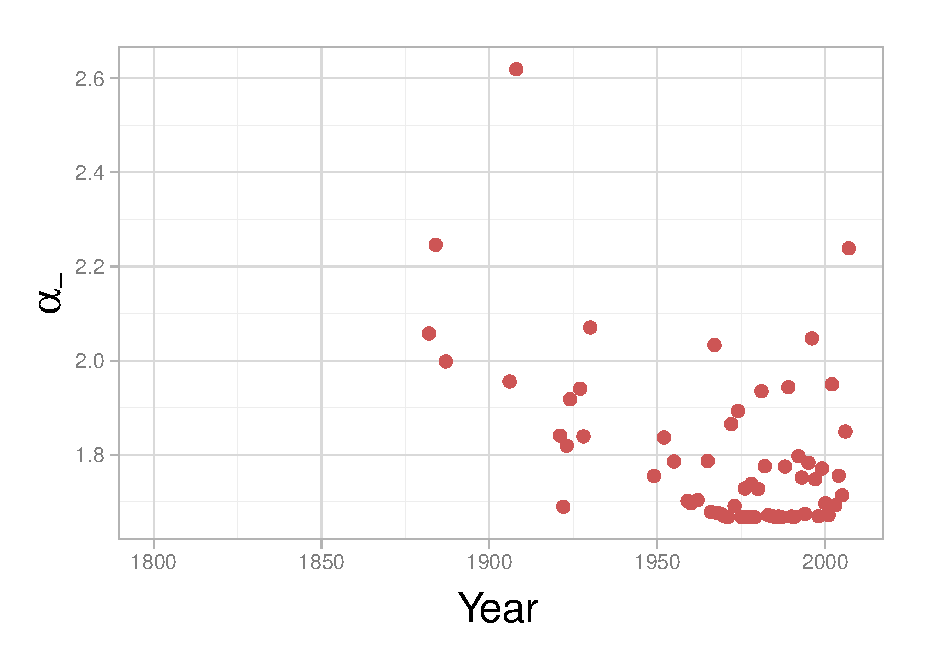
\includegraphics[width=0.9\linewidth]{alphamin.eps}
  \captionof{figure}{Evolution of $\alpha_{-}$ for English when calculated using all data outside the kernel lexicon. Only years for which the fit was statistically significant and with coefficient lower than 3 is shown. }
  \label{alphamin}
\end{minipage}%
\hfill%
\begin{minipage}[t]{.48\textwidth}
  \centering
  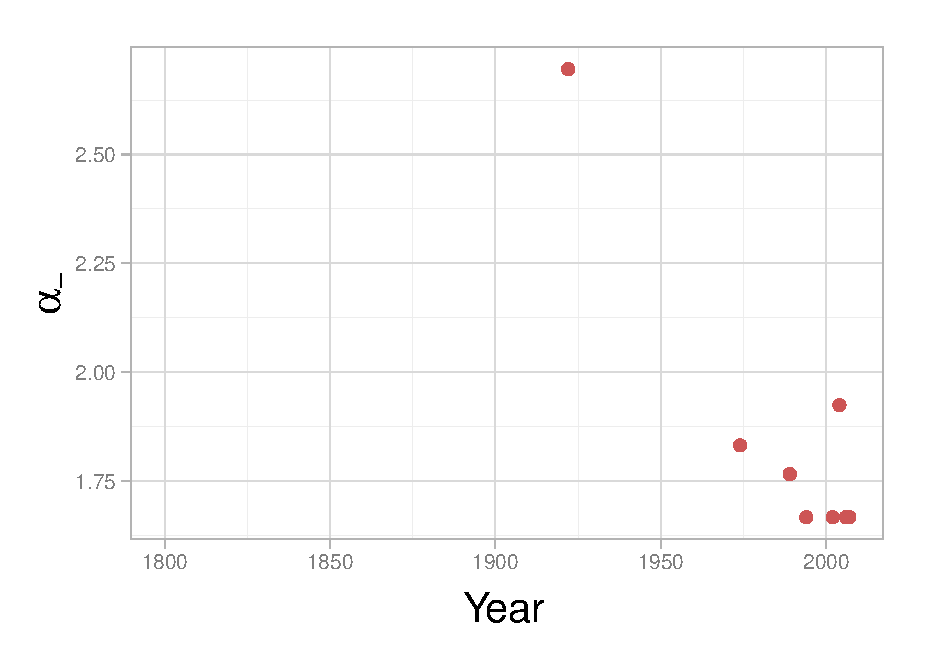
\includegraphics[width=0.9\linewidth]{alpha-5.eps}
  \captionof{figure}{Evolution of $\alpha_{-}$ for English when calculated using all data with relative frequencies below $10^{-5}$. Only years for which the fit was statistically significant and with coefficient lower than 3 is shown.}
  \label{alpha-5}
\end{minipage}
\end{figure}

However, when the data is plotted as in Figure \ref{Regimes} the kink appears clearly, and the data in the low frequency regime seems to be linear. Thus we opt for a final technique, we use a segmented linear regression method, proposed in a paper by \citeasnoun{segmented} to fit a histogram of the data. The algorithm automatically detects the kink and estimates the slopes of the two regimes. For a fixed number of breaks in the histogram this approach worked fine, giving sensible values for the coefficients and predicting a position of the kink consistent with that found in the previous section. However, we find that the number of breaks used to build the histogram changes the resulting coefficients in a noticeable way, rendering this method unreliable. If the whole dataset is used to produce the frequency density function instead of a histogram, the algorithm does not detect the kink correctly because of the noise generated by low frequency words.\\


The fact that any new addition to the lexicon enter as part of the unlimited lexicon makes it more variable and its analysis more challenging. However, this also implies that size effects can be stronger, with which extracting the desired information becomes harder. Thus our main focus of study remains to be the kernel lexicon, but we feel that other attempts at the study of the evolution of this lexicon are worth the effort. Two possible paths to follow are the construction of \textit{ad hoc} statistical tools for fitting this particular distribution or using a slightly different yet equally simple model to describe the data, such as the one presented by \citeasnoun{scaling}.\\       

 \section{Discussion}
 
 We found three interesting results: The power law coefficients are increasing, which means that the rank distribution is getting flatter; the size of the kernel lexicon remains constant, which supports the hypothesis of a relation of brain capacities with the structure of this lexicon; and the proportion of tokens in the kernel lexicon is decreasing, hence the unlimited lexicon is gaining relevance. Is there a plausible phenomenon that can account for all of this results and that is compatible with the general growth of types and tokens?\\
 
 We argue that an increase in the topicality of language, in this case of the scanned books, can be deemed a likely cause of the observed results. By this we do not necessarily mean an increase in the number of covered topics, but a more even distribution of language across existent topics. First of all, this would give more opportunities for topic specific words to be used and for more general words to be applied in different contexts, which would bring the frequencies of similarly ranked words closer. An example that this would be the case is given by analysing texts produced by people suffering schizophrenia \cite{Zipf}, \cite{schi}, \cite{zipf-variation}; it was found that people in early stages of schizophrenia, who tend to cover lots of different topics and change between them at a higher rate than normal, produced documents with $\alpha_{+}>2$. On the other hand, patients in advanced stages, who become obsessed with one topic, generated language with $\alpha_{+}<2$. This instance does not prove that our hypothesis is correct, but it gives hints that it can at least explain part of the registered phenomena.  \\
 
 Moreover, an increase in topicality would boost the use and size of the unlimited lexicon, since more specific vocabulary would be needed, thus incrementing the overall number of types and the proportion of tokens belonging to the unlimited lexicon. Although the presence of more topics or a more frequent treatment of them would also yield more instances of words in the kernel lexicon, it is likely that these increments would occur in a fixed and slower rate than in the unlimited lexicon, since the general words could not deal with the intricacies of specific topics and any new word needed would automatically increase the numbers of the latter lexicon. On the other hand, the necessary use of the basic words in the kernel lexicon across all topics would permit the division between lexicons to be preserved, in a way that would stop words from switching from the unlimited lexicon to the kernel lexicon. Besides, if a physical constraint is in play, the structure of languages would depend on it, thus making the existence of the kernel lexicon an inherent emergent property that cannot be challenged by changes within the language.\\
 
 This hypothesis can be tested by constructing a model that reproduces the known statistical features of language and makes falsifiable predictions. We propose a simple idea for further study, a minimal model that could capture the changing behaviour of the power law coefficient while giving information on the possible behavior of another measurable feature of language. Text can be generated using a Markov chain with a transition matrix selected a priori to produce frequencies distributed according to a power law and in such a way that changes in topicality can be introduced, for example by having classes representing topics. In this way Zipf's law would be obtained by construction, which is not optimal if the objective is to generate realistic text. However, the idea behind this basic model is to study whether topicality can explain part of the variation seen in the data, not to make a plausible model for language. It can be argued that such a model is not related to language whatsoever, since the text could be considered just a sequence of colored balls. Nevertheless, the objective is precisely to know if changes in topicality itself, which in the context of balls could be considered clustering (understanding topics and its words as clusters of balls), could yield results similar to the ones found in empirical studies of real texts. That is, this model would permit us study whether and important factor in topicality, the way it clusters words, can affect the features of interest without the need of additional considerations of language structure.
Since Zipf's law is being obtained by construction, the results to test would be statistics on pairs of adjacent words, which can be contrasted with the Google 2-grams.\\  
 
 
 
 \section{Conclusions and perspectives}
 
 The number of published texts has grown exponentially over the last centuries, giving the possibility of large scale studies of language. The sheer increase in the number of used types and tokens in written documents is an example of language evolution, although changes in structural levels are more interesting. Statistical properties of language are also evolving, specifically Zipf's coefficient, whose decreasing trend is highly correlated with the growth of the number of words in documents. Nonetheless, not all the variation can be explained by this correlations, which suggests changes on deeper levels. \\
 
There exists a relatively  small kernel lexicon of common words for each language, whose size remains fairly constant. This fact can be explained if the origin of the kernel lexicon is found in mental constraints and the way our brain renders language. However, the relative size of this kernel lexicon with respect to the unlimited lexicon, i.e. the rest of the words, is decreasing linearly, yielding a continual increment in the relevance of the unlimited lexicon.\\
 
 An evolution of the structure of language or of how it is used is likely to be taking place and producing changes in the power law behavior of word frequencies and in the relations between kernel and unlimited lexicons. One possibility is the increment of topicality in modern times, with many new topics emerging carrying their own vocabulary, and with the interrelation between topics becoming richer, which could lead to a more even distribution of words across different topics. The constant need of new words to cover the emerging topics would explain the terrain gained by the unlimited lexicon.\\
 
 The heuristic to build a Markov chain model that can be used to investigate the effects of topicality on language statistics will be put into practice in subsequent work. Furthermore, languages outside the Indo-European family should be analysed to compare the changes that have been found for the six European languages studied. An improvement in the statistical methods for fitting power laws could open the possibility of a thorough analysis of the coefficient $\alpha_{-}$, similar to what has been done  for 
 $\alpha_{+}$. It is also of interest to apply the approach of \cite{lemmas} regarding the study of lemmas instead of complete words, since this could show different patterns of evolution. The limitations for all the ideas related with analysis of language evolution are centered mainly on the availability of data, since it is a gargantuan task to digitize documents in the amounts required to cover a decent timespan, with enough data per period of interest. Hence any effort put towards that objective would open many more possibilities for the study of human language, culture and knowledge in general.\\
 

\section*{Acknowledgements}

I am really grateful to my supervisor Thomas Hills for his constant support and insightful ideas. I also want to thank the feedback given by colleagues and professors, specially the people attending the oral presentation of this project. Finally I want to express my gratitude towards the people involved in the Centre of Complexity Science and the Erasmus Mundus Program for the opportunities that I have received throughout this year.\\



 \bibliography{exportados}
 
\end{document}  